% !TeX root = ../thesis.tex
\chapter{Kết quả và thảo luận}
\label{chap:results}

Chương này đánh giá PE-GH theo những câu hỏi đã đặt ra, đồng thời phân biệt ba phạm vi bằng chứng. Kết quả xác nhận chính sử dụng sáu miền chưa tham gia lựa chọn phương pháp tại thời điểm đăng ký. Phép đo trên Programmers và Unix kiểm tra chất lượng đi kèm chi phí phục vụ truy vấn. Đối chiếu BERT và LiteGator được thực hiện sau đó theo phân tích thăm dò. Các kết quả được trình bày riêng theo phạm vi dữ liệu và điều kiện đánh giá.

\section{Chất lượng truy xuất trên các miền xác nhận}
\subsection{Mức chất lượng của các lựa chọn truy xuất}
Trước khi xem xét bộ quyết định, cần xác định hai nhánh có tạo ra một bài toán lựa chọn đáng kể hay không. Bảng~\ref{tab:quality} cho thấy \Hstar{} đạt \ndcg{} trung bình macro 0,4223, cao hơn BM25 0,3267 và Dense độc lập 0,4031. Trong phạm vi này, chạy cả hai nguồn mang lại lợi ích so với chỉ dùng từ khóa hoặc chỉ dùng ngữ nghĩa. Vì vậy, việc bỏ qua Dense có một chi phí chất lượng tiềm tàng thực sự, không chỉ bỏ một nhánh gần như vô ích.

\begin{table}[htbp]
\centering\small
\caption{Chất lượng trên sáu miền xác nhận. Dòng vận hành phản ánh chính sách đã chốt, còn dòng so khớp 50\% dùng cùng số lượt Dense với các đối chứng lựa chọn truy vấn.}
\label{tab:quality}
% Sinh bởi tools/prepare_evidence.py từ report/evidence.
\begin{tabularx}{\textwidth}{@{}Yrr@{}}
\hline
Phương pháp & \ndcg & Dense (\%) \\\hline
BM25 & 0,3267 & 0 \\
\Pstar & 0,3270 & 0 \\
Dense arctic & 0,4031 & 100 \\
\Hstar & 0,4223 & 100 \\
PE-GH v2 vận hành & 0,4159 & 80 \\
PE-GH v2 so khớp & 0,3933 & 50 \\
BM25-margin & 0,3892 & 50 \\
Ngẫu nhiên & 0,3744 & 50 \\
PE-GH v1 & 0,3469 & 81,8 \\
\hline
\end{tabularx}

\source{Thực nghiệm xác nhận của nhóm trên sáu miền CQADupStack}
\end{table}

Nhánh \Pstar{} đạt 0,3270, chỉ cao hơn điểm BM25 khoảng 0,0003. Quan sát này cho thấy phần xếp hạng bổ sung trong hệ cuối chưa mang lại cải thiện trung bình đáng kể về mặt độ lớn trên các miền xác nhận. Tuy nhiên, hai giá trị trung bình gần nhau chưa chứng minh hai nhánh tương đương bằng một phép kiểm định. Cách diễn giải phù hợp là lợi ích quan sát của phần xếp hạng bổ sung nhỏ, nên cần cân nhắc phần chi phí mà nó thêm vào nhánh được kỳ vọng là rẻ.

Ở ngân sách vận hành 80\%, PE-GH v2 đạt 0,4159, thấp hơn \Hstar{} khoảng 0,0064. Chất lượng không được giữ nguyên hoàn toàn, nhưng mức suy giảm nhỏ hơn biên 0,01 mà đề tài chấp nhận trước xác nhận. Đổi lại, tỷ lệ thực tế sử dụng Dense nằm khoảng 79,9\% đến 80,2\% theo miền. Kết quả này hỗ trợ cách sử dụng PE-GH như một lựa chọn đánh đổi có kiểm soát, thay vì một phương pháp đạt toàn bộ chất lượng Hybrid mà không trả chi phí tương ứng.

Tại ngân sách so khớp 50\%, chất lượng PE-GH là 0,3933. Điểm này thấp hơn mức vận hành 80\%, nhưng cho phép xem rõ hơn giá trị của thứ tự ưu tiên truy vấn. Với cùng số lượt Dense, BM25-margin đạt 0,3892 và lựa chọn ngẫu nhiên đạt 0,3744. Khoảng chênh lệch với ngẫu nhiên lớn hơn khoảng chênh lệch với margin. Vì vậy, có khả năng lựa chọn hữu ích không đồng nghĩa mô hình học tạo ra một bước tiến lớn so với một quy tắc rẻ đã có tín hiệu tốt.

\subsection{Sự thay đổi theo miền}
\begin{table}[htbp]
\centering\small
\caption{Chất lượng theo miền và chênh lệch giữa PE-GH v2 với margin ở cùng ngân sách 50\%. Các giá trị là mô tả, chưa phải kiểm định riêng cho từng miền.}
\label{tab:domains}
% Sinh bởi tools/prepare_evidence.py từ report/evidence.
\begin{tabularx}{\textwidth}{@{}Yrrrr@{}}
\hline
Miền & BM25 & \Hstar & V2 (80\%) & V2 $-$ margin (50\%) \\\hline
English & 0,3375 & 0,4590 & 0,4505 & 0,0014 \\
Gaming & 0,4675 & 0,5863 & 0,5815 & 0,0082 \\
Physics & 0,3266 & 0,4388 & 0,4310 & 0,0055 \\
Stats & 0,2883 & 0,3624 & 0,3571 & 0,0139 \\
Tex & 0,2490 & 0,3185 & 0,3179 & 0,0035 \\
Wordpress & 0,2914 & 0,3686 & 0,3574 & -0,0074 \\
\hline
\end{tabularx}

\source{Thực nghiệm xác nhận của nhóm; kết quả tổng hợp theo miền}
\end{table}

Bảng~\ref{tab:domains} cho thấy mức chất lượng khác nhau đáng kể giữa các miền. Gaming có điểm Hybrid cao hơn các miền còn lại, trong khi TeX thấp hơn dù chứa nhiều truy vấn hơn. Do báo cáo dùng macro theo miền, sự chênh lệch số truy vấn không làm TeX có trọng số cao hơn Gaming trong kết quả chính. Cách tổng hợp này giữ câu hỏi nghiên cứu ở mức hiệu quả trung bình trên các cộng đồng, thay vì chỉ trên một truy vấn lấy ngẫu nhiên từ tập gộp.

PE-GH v2 hơn margin ở năm trong sáu miền tại 50\%. WordPress là ngoại lệ, với chênh lệch khoảng $-0{,}0074$. Stats có mức chênh dương lớn nhất, khoảng 0,0139. Các giá trị này cho biết lợi thế trung bình không phân bố đồng đều và không bảo đảm mọi miền được cải thiện. Do chưa có phép kiểm định riêng đã đăng ký cho từng miền, báo cáo dùng chúng để phân tích sự không đồng nhất, không xem mỗi dấu dương là một phát hiện xác nhận độc lập.

Ở ngân sách 80\%, WordPress còn có mức giảm so với \Hstar{} khoảng 0,0112, lớn hơn biên 0,01 nếu chỉ nhìn điểm trung bình miền. K2 vẫn là giả thuyết trên macro sáu miền, nên kết quả đạt K2 không bảo đảm từng miền đều thỏa cùng một biên. Đây là khác biệt có ý nghĩa khi triển khai: một đơn vị vận hành chỉ quan tâm WordPress không thể dùng kết luận macro để bỏ qua mức mất mát riêng của miền đó.

\section{Kiểm chứng các giả thuyết nghiên cứu}
\begin{table}[htbp]
\centering\small
\caption{Kết quả K1 đến K4 trên sáu miền xác nhận. Cột khoảng tin cậy dùng hai phía để mô tả, còn quyết định kiểm định dùng p-value một phía và Holm theo giao thức.}
\label{tab:hypotheses}
% Sinh bởi tools/prepare_evidence.py từ report/evidence.
\begin{tabularx}{\textwidth}{@{}Yrrrl@{}}
\hline
Giả thuyết & Chênh lệch & CI hai phía 95\% & $p$ một phía & Holm \\\hline
K1 & 0,0042 & [0,0003; 0,0081] & 0,0171 & Đạt \\
K2 & -0,0064 & [-0,0085; -0,0043] & 0,0009 & Đạt \\
K3 & 0,0690 & [0,0629; 0,0752] & $<0{,}0001$ & Đạt \\
K4 & 0,0190 & [0,0155; 0,0225] & $<0{,}0001$ & Đạt \\
\hline
\end{tabularx}

\source{Thực nghiệm của nhóm; khoảng tin cậy được ước lượng bằng lấy mẫu lại theo nhóm truy vấn}
\end{table}

K1 cho chênh lệch PE-GH v2 trừ BM25-margin khoảng 0,0042 tại cùng ngân sách 50\%, với khoảng tin cậy hai phía 95\% từ 0,0003 đến 0,0081. P-value một phía là 0,0171 và phép kiểm định đạt điều kiện Holm. Kết quả hỗ trợ giả thuyết bộ quyết định học có giá trị riêng trên các miền xác nhận. Tuy nhiên, cận dưới gần 0 và độ lớn cải thiện nhỏ cho thấy cần trình bày hiệu ứng đúng mức, thay vì mô tả như một bước tăng chất lượng lớn.

K2 có chênh lệch so với \Hstar{} khoảng $-0{,}0064$. Cận dưới một phía 95\% là khoảng $-0{,}00819$, nằm phía trên $-0{,}01$, đồng thời phép kiểm định không kém đạt điều kiện Holm. Kết luận được hỗ trợ là PE-GH ở điểm vận hành giảm số lượt Dense mà không kém mốc Hybrid quá biên đã đăng ký. Khoảng tin cậy hai phía của chênh lệch nằm hoàn toàn dưới 0, nên bằng chứng cũng cho thấy tồn tại một mức giảm chất lượng đo được. Hai nhận định này nhất quán vì mục tiêu không kém cho phép mất mát hữu hạn.

K3 ghi nhận v2 cao hơn v1 khoảng 0,0690, với khoảng tin cậy từ 0,0629 đến 0,0752. Chênh lệch này lớn hơn đáng kể hiệu ứng K1 nhưng thuộc so sánh toàn hệ thống. V2 sử dụng mô hình ngữ nghĩa khác, nhánh truy xuất khác và mục tiêu học khác. Do đó, kết quả cho biết phiên bản cuối phù hợp hơn trong giao thức so sánh đã dùng, chưa chứng minh riêng thay đổi bộ quyết định đã tạo ra toàn bộ cải thiện.

K4 cho mức hơn lựa chọn ngẫu nhiên khoảng 0,0190 tại cùng ngân sách 50\%, với khoảng tin cậy từ 0,0155 đến 0,0225. Kết quả này xác nhận bộ quyết định không chỉ đạt chất lượng do phân bổ tài nguyên tùy ý. Đặt cạnh K1, nó cũng cho thấy margin đã khai thác được một phần lớn tín hiệu hữu ích. Giá trị cần đánh giá của mô hình học là phần cải thiện bổ sung trước đối chứng này, không phải toàn bộ khoảng cách từ ngẫu nhiên lên PE-GH.

\begin{figure}[htbp]
\centering
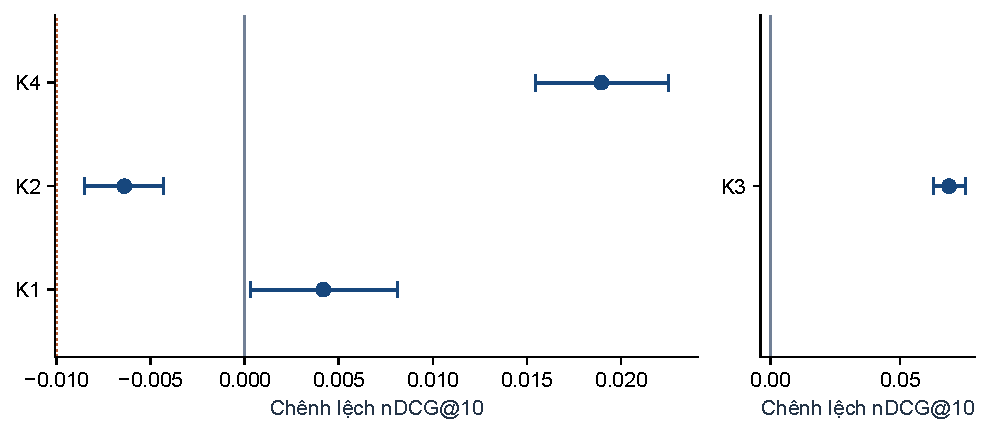
\includegraphics[width=\textwidth]{hypotheses.pdf}
\caption{Ước lượng và khoảng tin cậy hai phía 95\% của K1 đến K4. K3 dùng ô riêng vì độ lớn khác biệt. Đường tại $-0{,}01$ minh họa biên của K2; kết luận K2 dùng cận một phía và kiểm định đã hiệu chỉnh.}
\label{fig:hypotheses}
\end{figure}

Cả bốn giả thuyết đạt tiêu chí trong phạm vi xác nhận, nhưng chúng trả lời những câu hỏi khác nhau. K1 và K4 liên quan trực tiếp đến việc lựa chọn truy vấn. K2 đánh giá một điểm vận hành của chính sách. K3 đánh giá mức nâng cấp cả hệ thống. Việc tách vai trò giúp tránh dùng kết quả mạnh của K3 để làm lớn hơn đóng góp riêng của bộ quyết định hoặc dùng K2 để khẳng định chất lượng được giữ nguyên.

\section{Quan hệ giữa chất lượng và chi phí}
\subsection{Độ trễ đầu cuối và tỷ lệ sử dụng Dense}
\begin{table}[htbp]
\centering\small
\caption{Phiên online chính trên Programmers và Unix. Mean, p95 và CPU tính bằng ms; RSS là bộ nhớ đỉnh tính bằng MiB. Chất lượng là macro hai miền, khác phạm vi sáu miền của Bảng~\ref{tab:quality}.}
\label{tab:online}
% Sinh bởi tools/prepare_evidence.py từ report/evidence.
\begin{tabularx}{\textwidth}{@{}Yrrrrr@{}}
\hline
Phương pháp & Mean & p95 & CPU & RSS & \ndcg \\\hline
BM25 & 2,03 & 3,51 & 2,0 & 285,4 & 0,2899 \\
\Pstar & 3,49 & 5,06 & 3,5 & 620,4 & 0,2952 \\
\Rstar & 14,70 & 17,66 & 57,5 & 654,3 & 0,3811 \\
\Hstar & 24,31 & 28,95 & 90,7 & 726,0 & 0,4142 \\
PE-GH v2 (30\%) & 10,68 & 26,77 & 39,3 & 768,0 & 0,3428 \\
PE-GH v2 (50\%) & 14,76 & 28,14 & 54,5 & 769,3 & 0,3745 \\
PE-GH v2 (80\%) & 20,98 & 29,52 & 78,5 & 771,3 & 0,4107 \\
\hline
\end{tabularx}

\source{Phiên online chính của nhóm; 9.740 yêu cầu cho mỗi phương pháp}
\end{table}

Trong phiên online chính, \Hstar{} có độ trễ trung bình 24,31 ms. PE-GH v2 ở ngân sách 50\% đạt 14,76 ms, giảm khoảng 39,3\%, với khoảng tin cậy 95\% của mức giảm từ 37,5\% đến 41,1\%. Tỷ lệ Dense thực tế khoảng 50,1\%. Số đo xác nhận việc bỏ qua Dense chuyển thành lợi ích thời gian trong điều kiện đã đo, nhưng mức giảm thời gian thấp hơn mức giảm số lượt Dense vì hệ thống vẫn trả chi phí BM25, bộ quyết định và nhánh rẻ.

Ở mức 30\%, độ trễ trung bình giảm còn 10,68 ms, đi kèm chất lượng 0,3428. Ở mức 80\%, độ trễ là 20,98 ms và chất lượng 0,4107. Những điểm này không nên được xếp thành một kết luận duy nhất rằng ngân sách càng thấp càng tốt. Người vận hành nhận được thời gian thấp hơn bằng cách chấp nhận sử dụng Dense ít hơn, trong khi chất lượng có thể giảm. Ý nghĩa của ngân sách là làm rõ lựa chọn đó, không xóa bỏ đánh đổi.

Điểm 80\% có ý nghĩa riêng đối với mục tiêu giữ chất lượng Hybrid. Trong phiên chính, mức giảm độ trễ trung bình so với \Hstar{} khoảng 13,7\%, nhỏ hơn đáng kể mức 39,3\% ở 50\%. Vì vậy, không thể ghép kết luận chất lượng của điểm 80\% với mức tăng tốc ở 50\% để mô tả một hệ thống duy nhất. Trên sáu miền xác nhận, K2 thuộc 80\%; trên hai miền online, số đo của mỗi điểm phải đi cùng chất lượng và tỷ lệ Dense tương ứng.

\begin{figure}[htbp]
\centering
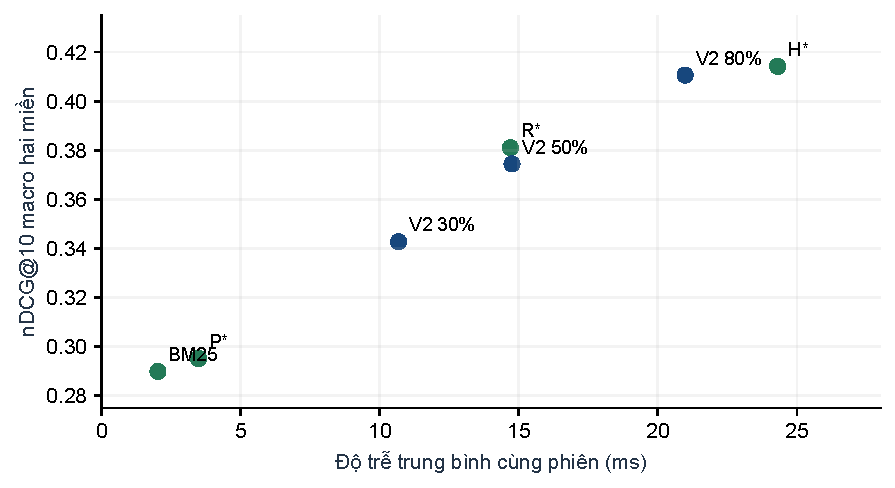
\includegraphics[width=\textwidth]{online_tradeoff.pdf}
\caption{Chất lượng và độ trễ trung bình của các phương pháp trong cùng phiên online chính. Các điểm là kết quả quan sát trên hai miền, không phải dự đoán thời gian từ tỷ lệ Dense.}
\label{fig:online}
\end{figure}

\subsection{Chi phí hai nhánh và độ trễ đuôi}
Lợi ích về độ trễ trung bình xuất hiện khi một phần truy vấn được kết thúc ở nhánh chi phí thấp. Những truy vấn này không cần thực hiện thêm toàn bộ quá trình truy xuất ngữ nghĩa. Tuy nhiên, các truy vấn được chuyển sang Hybrid vẫn phải thực hiện phần công việc có chi phí cao hơn. Vì vậy, thời gian trung bình có thể giảm trong khi thời gian của nhóm yêu cầu chậm nhất thay đổi ít.

p95 của \Hstar{} là 28,95 ms, trong khi PE-GH ở 50\% là 28,14 ms và ở 80\% là 29,52 ms. Không có một xu hướng cải thiện đuôi rõ ràng tương ứng với mức giảm độ trễ trung bình. Những yêu cầu đi nhánh Dense vẫn chịu chi phí mã hóa và tìm vector, cộng thêm phần quyết định. Khi nhóm yêu cầu chậm nằm chủ yếu ở nhánh này, bỏ qua Dense cho các truy vấn khác không làm p95 giảm nhiều.

Kết quả p95 cũng cho thấy yêu cầu vận hành cần được xác định trước khi chọn phương pháp. Nếu ưu tiên là giảm tổng tài nguyên xử lý hoặc độ trễ trung bình, bỏ qua Dense có thể hữu ích. Nếu ưu tiên là thời gian phản hồi ổn định cho gần như mọi yêu cầu, chỉ thêm bộ quyết định chưa giải quyết được vấn đề. Khi đó, cần cải thiện cả những yêu cầu vẫn sử dụng Dense, thay vì kỳ vọng giảm số lượt sử dụng nhánh này sẽ cải thiện mọi khía cạnh của thời gian phản hồi.

Thời gian CPU trung bình của PE-GH 50\% khoảng 54,5 ms, thấp hơn \Hstar{} khoảng 90,7 ms trong cùng phiên. Đại lượng này phản ánh tài nguyên xử lý đã sử dụng, còn độ trễ phản ánh thời gian chờ kết quả. Hai góc nhìn cùng hỗ trợ đánh giá lợi ích của phương pháp, nhưng chưa cho biết hệ thống sẽ phục vụ được bao nhiêu yêu cầu khi nhiều người dùng truy cập đồng thời.

Bộ nhớ đỉnh không giảm theo tỷ lệ bỏ qua Dense. Ở 50\%, PE-GH dùng khoảng 769 MiB, so với khoảng 726 MiB của \Hstar{}. Hệ thống vẫn phải sẵn sàng thực hiện truy xuất ngữ nghĩa khi được lựa chọn và còn sử dụng thêm bộ quyết định. Vì vậy, giảm số lượt Dense không đồng nghĩa giảm nhu cầu bộ nhớ. Kết quả hiện có hỗ trợ lợi ích về thời gian và tài nguyên xử lý, chưa hỗ trợ kết luận tiết kiệm bộ nhớ.

\subsection{Các lựa chọn cạnh tranh về chi phí}
\Rstar{} đạt khoảng 14,70 ms và chất lượng 0,3811, trong khi PE-GH 50\% đạt 14,76 ms và 0,3745 trên hai miền online. Hai điểm trung bình đặt cạnh nhau cho thấy chấm lại ứng viên BM25 là một đối chứng đáng chú ý tại vùng chi phí này. Chưa có kiểm định riêng trong bảng để kết luận \Rstar{} luôn tốt hơn, nhưng quan sát đủ để bác bỏ cách trình bày PE-GH như lựa chọn duy nhất đáng cân nhắc cho mọi mục tiêu thời gian.

\Rstar{} và PE-GH tiết kiệm ở những vị trí khác nhau. \Rstar{} mã hóa mọi truy vấn nhưng bỏ việc tìm kiếm vector trên toàn kho, còn PE-GH bỏ cả mã hóa và tìm vector cho một phần truy vấn. Do đó, phương án phù hợp phụ thuộc tương quan giữa chi phí mã hóa truy vấn, chi phí tìm vector và khả năng BM25 chứa tài liệu cần thiết trong tập ứng viên. Nếu chỉ dùng tỷ lệ sử dụng Dense làm đại diện toàn bộ chi phí, sự khác nhau này sẽ bị che khuất.

Nhánh \Pstar{} cũng cần được đối chiếu với BM25. Trong phiên đo chính, BM25 mất khoảng 2,03 ms và \Pstar{} khoảng 3,49 ms. Lợi ích chất lượng của \Pstar{} có tồn tại trên hai miền này, nhưng nhỏ hơn nhiều khoảng cách từ \Pstar{} đến \Hstar{}. Trên sáu miền xác nhận, phần xếp hạng bổ sung chỉ làm điểm trung bình tăng rất ít. Kết quả đặt ra câu hỏi liệu lợi ích đó có đủ để bù phần chi phí thêm vào nhánh được kỳ vọng là rẻ hay không.

\section{Khả năng lựa chọn truy vấn}
\subsection{Lợi ích thay đổi theo ngân sách}
\begin{figure}[htbp]
\centering
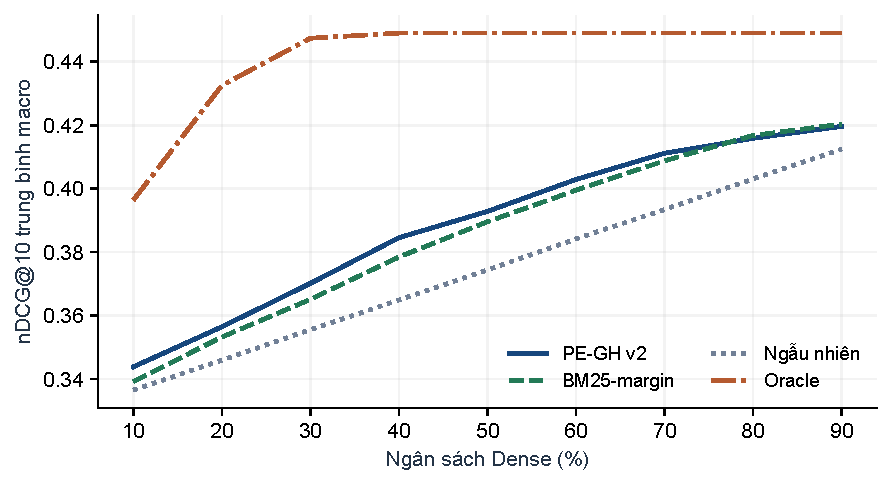
\includegraphics[width=\textwidth]{budget_curves.pdf}
\caption{Chất lượng theo ngân sách trên sáu miền xác nhận. Đường cong mô tả xu hướng và không thay thế kết quả kiểm định riêng của K1 và K2.}
\label{fig:budgets}
\end{figure}

Hình~\ref{fig:budgets} cho thấy lợi thế của PE-GH trước margin tập trung ở vùng ngân sách thấp và trung bình. Trong những điểm mô tả từ 10\% đến 70\%, PE-GH cao hơn margin khoảng 0,002 đến 0,006 \ndcg{}. Từ 80\% trở lên, điểm quan sát của margin nhỉnh hơn nhẹ. Đường cong vì thế không hỗ trợ một kết luận rằng bộ quyết định học có ưu thế ở mọi mức sử dụng Dense.

Khi ngân sách thấp, phương pháp phải chọn một tập nhỏ truy vấn đáng ưu tiên. Thứ tự điểm có thể tạo ra khác biệt rõ hơn trong vùng này. Khi ngân sách cao, phần lớn truy vấn đều đã được chuyển sang Hybrid, nên chỉ còn một nhóm nhỏ bị bỏ qua. Đây là một cách giải thích phù hợp với hình dạng đường cong, nhưng báo cáo không xem nó là bằng chứng trực tiếp rằng hai phương pháp đã chọn cùng một tập truy vấn. Kết luận về mức trùng tập lựa chọn cần bằng chứng về nhánh đã chọn cho từng truy vấn.

Điểm 50\% của đường cong cho PE-GH khoảng 0,3928, khác số 0,3933 trong K1. Tương tự, mốc vận hành 80\% là 0,4159, còn so khớp 80\% trong đối chiếu bộ quyết định là 0,4156. Các chênh lệch nhỏ này đến từ những quy tắc phân bổ trong hồ sơ tương ứng. Báo cáo giữ đúng giá trị của từng giao thức, bởi chọn một con số thay cho con số khác sẽ làm mất quan hệ giữa bằng chứng và phép kiểm chứng.

Oracle ở 50\% đạt khoảng 0,4490, trong khi PE-GH ở vùng này khoảng 0,393. Khoảng cách lớn cho thấy còn nhiều khả năng lựa chọn tốt hơn nếu biết chất lượng thực tế của hai nhánh. Oracle thậm chí có thể hơn luôn chạy Hybrid vì có thể tránh những truy vấn mà Hybrid làm giảm chất lượng. Tuy nhiên, nó sử dụng thông tin mà hệ thống phục vụ không có, nên không được diễn giải thành mức chất lượng có thể đạt ngay bằng một ngưỡng khác.

\subsection{Dự báo BM25 và lợi ích hành động}
PE-GH v2 có AUC dự đoán BM25 thất bại khoảng 0,764, so với khoảng 0,670 của margin trên sáu miền xác nhận. AUC của v2 cao hơn margin ở cả sáu miền. Đây là bằng chứng bộ quyết định sắp thứ tự rủi ro BM25 tốt hơn đối chứng theo mục tiêu dự báo đã chọn, nhưng mức cải thiện chất lượng truy xuất K1 vẫn chỉ khoảng 0,0042.

Sự khác biệt giữa hai mức hiệu quả phù hợp với giới hạn của nhãn học đã nêu ở Chương~\ref{chap:method}. Trong phân tích thăm dò, AUC của v2 đối với nhãn Hybrid có lợi hơn nhánh rẻ chỉ khoảng 0,570, thấp hơn AUC dự báo BM25 thất bại. Nhãn được dự đoán tốt hơn không hoàn toàn trùng với đại lượng quyết định chất lượng của nhánh được chọn. Do đó, báo cáo không dùng AUC 0,764 để thay cho bằng chứng rằng mọi truy vấn được ưu tiên đều hưởng lợi từ Dense.

\begin{figure}[htbp]
\centering
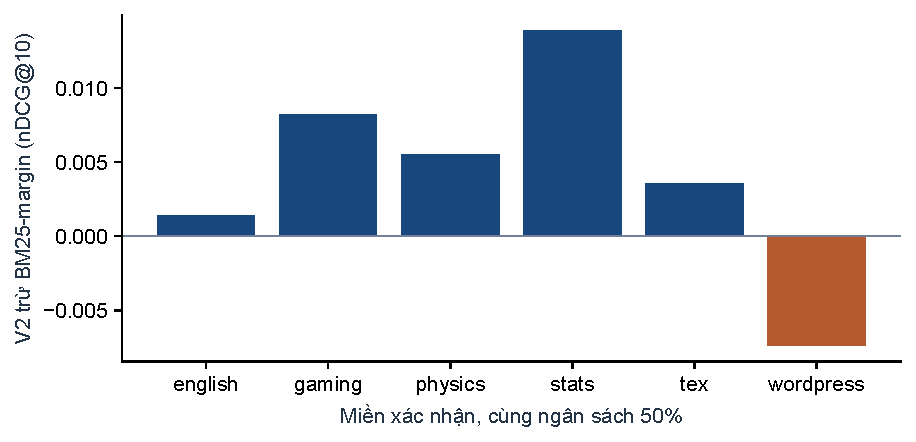
\includegraphics[width=\textwidth]{per_domain_gains.pdf}
\caption{Chênh lệch v2 trừ margin theo miền ở cùng ngân sách 50\%. WordPress có chênh lệch âm dù AUC dự báo BM25 của v2 cao hơn margin.}
\label{fig:domain-gain}
\end{figure}

Các so sánh thăm dò còn cho thấy một bộ quyết định dùng ít thông tin hơn vẫn có thể đạt chất lượng gần bản đầy đủ. Thay mục tiêu học sang nhận biết BM25 thất bại cũng đem lại kết quả đáng chú ý trong những phương án được thử. Những quan sát này gợi ý rằng lựa chọn điều cần dự báo có thể quan trọng hơn việc tăng độ phức tạp. Tuy nhiên, các thay đổi chưa được tách biệt hoàn toàn, nên báo cáo chưa quy phần cải thiện cho một nguyên nhân riêng.

Kết quả cần được dùng để giới hạn mô tả đóng góp. Bộ quyết định v2 là cấu hình đã được xác nhận trước margin trong đề tài, nhưng hiệu ứng nhỏ và phụ thuộc ngân sách. Giá trị phương pháp nằm ở việc chứng minh một cách lựa chọn hữu ích trong điều kiện cụ thể, cùng khả năng chỉ ra khi nào tín hiệu dự báo chưa chuyển thành lợi ích hành động.

\section{Đối chiếu các bộ quyết định liên quan}
\subsection{Chất lượng trên sáu miền xác nhận}
\begin{table}[htbp]
\centering\small
\caption{So sánh thăm dò các bộ quyết định ở cùng số lượt Dense. Tất cả dùng cùng hai nhánh truy xuất. Điểm 80\% ở đây thuộc phép so khớp ngân sách, khác điểm vận hành 80\% của K2.}
\label{tab:router-quality}
% Sinh bởi tools/prepare_evidence.py từ report/evidence.
\begin{tabularx}{\textwidth}{@{}Yrrr@{}}
\hline
Bộ quyết định & 30\% & 50\% & 80\% \\\hline
PE-GH v2 & 0,3698 & 0,3933 & 0,4156 \\
LiteGator mặc định & 0,3671 & 0,3904 & 0,4172 \\
LiteGator chọn cấu hình & 0,3678 & 0,3913 & 0,4169 \\
BERT điều chỉnh & 0,3697 & 0,3924 & 0,4224 \\
BM25-margin & 0,3648 & 0,3892 & 0,4172 \\
\hline
\end{tabularx}

\source{Đối chiếu thăm dò của nhóm trên sáu miền xác nhận}
\end{table}

Ở 30\% và 50\%, các điểm trung bình của PE-GH, BERT và LiteGator khá gần nhau. Tại 50\%, PE-GH đạt 0,3933, bản LiteGator mặc định đạt 0,3904 và BERT đạt 0,3924. Khoảng tin cậy hai phía của chênh lệch với hai bộ quyết định này chứa 0 trong phân tích thăm dò. Do đó, bằng chứng chưa đủ để khẳng định PE-GH có chất lượng cao hơn hai phiên bản điều chỉnh, đồng thời cũng chưa chứng minh chúng tương đương.

Tại 80\%, BERT đạt 0,4224, cao hơn PE-GH 0,4156. Chênh lệch PE-GH trừ BERT khoảng $-0{,}0068$, với khoảng tin cậy hai phía từ $-0{,}0094$ đến $-0{,}0044$. Đây là kết quả bất lợi cần được giữ trong đánh giá phương pháp. Việc PE-GH rẻ hơn về quyết định không xóa bỏ khả năng một bộ quyết định đắt hơn có chất lượng tốt hơn tại một ngân sách cụ thể.

Bản LiteGator được lựa chọn trên các miền phát triển đạt 0,3913 ở 50\%, so với 0,3904 của bản mặc định. Ở 80\%, bản được lựa chọn đạt 0,4169, cao hơn điểm trung bình của PE-GH nhưng khoảng tin cậy chênh lệch còn chứa 0. Giữ cả hai bản giúp tránh so phương pháp của nhóm đã qua lựa chọn với một đối chứng chưa được xem xét phương án phù hợp. Tuy vậy, BERT chưa được khảo sát nhiều phương án ở cùng mức, nên phép đối chiếu vẫn có giới hạn về cân bằng chi phí phát triển.

\subsection{Chi phí online trong phiên đối chiếu riêng}
\begin{table}[htbp]
\centering\small
\caption{Phiên đo đối chiếu bộ quyết định trên Programmers và Unix ở ngân sách 50\%. LiteGator là bản được lựa chọn trên dữ liệu phát triển; các phương án được đo trong cùng điều kiện và cùng phiên.}
\label{tab:router-online}
% Sinh bởi tools/prepare_evidence.py từ report/evidence.
\begin{tabularx}{\textwidth}{@{}Yrrr@{}}
\hline
Bộ quyết định (50\%) & Mean (ms) & p95 (ms) & \ndcg \\\hline
PE-GH v2 & 14,30 & 26,98 & 0,3736 \\
LiteGator chọn cấu hình & 14,43 & 27,56 & 0,3674 \\
BERT điều chỉnh & 162,57 & 264,86 & 0,3692 \\
\hline
\end{tabularx}

\source{Phiên online đối chiếu bộ quyết định của nhóm}
\end{table}

Trong phiên đối chiếu, PE-GH 50\% đạt độ trễ trung bình 14,30 ms, LiteGator 14,43 ms và BERT 162,57 ms. Phần chi phí của BERT lớn hơn rõ rệt so với hai mô hình nhẹ, và thậm chí lớn hơn mốc luôn chạy Hybrid khoảng 23,11 ms trong chính phiên này. Như vậy, một bộ quyết định có thể hữu ích về thứ tự lựa chọn nhưng không phù hợp với mục tiêu giảm chi phí CPU trong cấu hình phục vụ đang xét.

\begin{figure}[htbp]
\centering
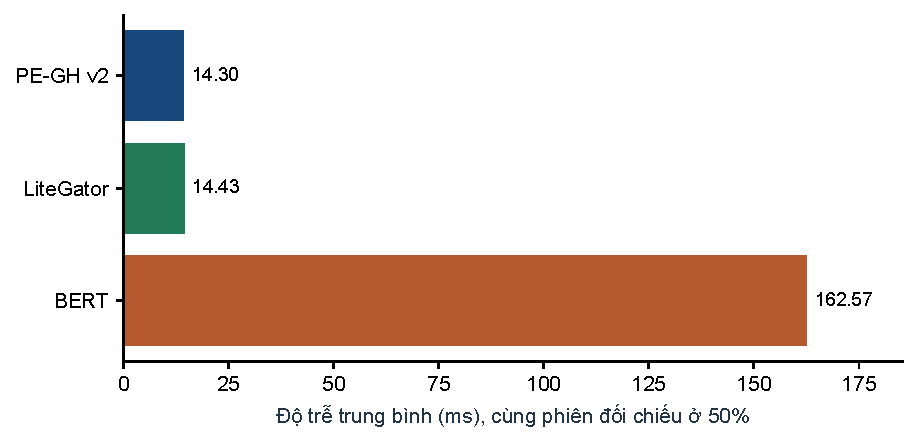
\includegraphics[width=\textwidth]{router_latency.pdf}
\caption{Độ trễ trung bình của ba bộ quyết định ở ngân sách 50\% trong phiên đối chiếu riêng. Hình thể hiện chi phí quan sát, không suy rộng tỷ lệ tăng tốc sang phần cứng khác.}
\label{fig:router-latency}
\end{figure}

Chênh lệch chất lượng PE-GH trừ BERT ở 50\% khoảng 0,0043, với CI hai phía từ $-0{,}0039$ đến 0,0125. Vì khoảng này chứa 0, so sánh chưa phát hiện khác biệt chất lượng theo cách đọc khoảng tin cậy đang dùng. Cùng lúc, chênh lệch độ trễ trung bình khoảng $-148{,}27$ ms có khoảng tin cậy từ $-150{,}65$ đến $-145{,}86$ ms. Hai bằng chứng hỗ trợ nhận định PE-GH rẻ hơn rõ trong phiên này mà chưa cho thấy khác biệt chất lượng rõ, nhưng chưa chứng minh hai bộ quyết định tương đương chất lượng.

Với LiteGator 50\%, PE-GH có chênh lệch chất lượng khoảng 0,0061, CI hai phía từ $-0{,}0003$ đến 0,0127. Chênh lệch mean khoảng $-0{,}13$ ms có CI từ $-0{,}55$ đến 0,27 ms. Các khoảng hai phía đều chứa 0, nên chưa có bằng chứng rõ rằng PE-GH cải thiện cả chất lượng lẫn tốc độ trước đối chứng nhẹ này. Kết quả làm hẹp phạm vi kết luận phù hợp: đề tài chứng minh lợi ích trước margin theo K1, chưa chứng minh thắng LiteGator về mọi đại lượng.

Phiên đối chiếu sử dụng mô hình được lựa chọn mà không có miền đang đo; các phương án được đánh giá trong điều kiện chung. Kết quả có cơ sở để so sánh bên trong phiên này, nhưng khoảng tin cậy chưa lượng hóa biến động giữa các máy hoặc nhiều phiên vận hành độc lập. Do đó, mức chênh lệch thời gian với BERT chỉ được gắn với phép đo CPU đã thực hiện.

\section{Các trường hợp chưa đáp ứng kỳ vọng}
\subsection{WordPress và giới hạn của kết quả trung bình}
WordPress là trường hợp rõ nhất cho thấy lợi ích macro không bảo đảm lợi ích từng miền. Ở cùng ngân sách 50\%, v2 đạt khoảng 0,3303 trong khi margin đạt 0,3377. AUC BM25 của v2 tại miền này vẫn khoảng 0,772, cao hơn margin khoảng 0,685. Hai quan sát cùng tồn tại cho thấy dự báo đúng hơn một biến liên quan chưa bảo đảm phân bổ ngân sách tốt hơn cho chất lượng cuối cùng.

Ở ngân sách vận hành 80\%, WordPress đạt khoảng 0,3574 so với \Hstar{} 0,3686. Mức giảm điểm trung bình khoảng 0,0112 đặt ngoài biên 0,01 nếu xét riêng miền. Giao thức không đặt K2 riêng cho WordPress, nên đây là một giới hạn triển khai rút ra từ mô tả, không phải một phép kiểm định xác nhận mới. Trong sử dụng cho một cộng đồng cụ thể, cần xác định lại tiêu chí chất lượng của cộng đồng đó thay vì dựa hoàn toàn vào kết luận macro.

\subsection{TeX và sự khác nhau giữa mức chất lượng và mức mất mát}
TeX có 2.906 truy vấn, là miền lớn nhất trong nhóm xác nhận. Điểm \Hstar{} khoảng 0,3185, thấp hơn các miền như English hoặc Gaming, nhưng PE-GH 80\% đạt khoảng 0,3179 và chỉ mất khoảng 0,0006. Một miền có điểm tuyệt đối thấp vì thế chưa chắc là miền bị lựa chọn nhánh làm tổn hại nhiều nhất. Cần phân biệt hạn chế của cả hai retriever với phần chất lượng mất thêm do bộ quyết định.

Nếu chỉ trình bày điểm tuyệt đối hoặc chỉ trình bày độ giảm, người đọc có thể có hai ấn tượng không đầy đủ về TeX. Báo cáo giữ đồng thời cả hai để cho thấy mục tiêu lựa chọn là kiểm soát mất mát trước một mốc Hybrid xác định, còn việc nâng chất lượng của chính mốc đó là một vấn đề khác. Quan sát này cũng giải thích vì sao chỉ tối ưu bộ quyết định chưa đủ giải quyết toàn bộ những miền khó.

\subsection{Ảnh hưởng của chất lượng các nhánh truy xuất}
\begin{table}[htbp]
\centering\small
\caption{Các phương án mô hình ngữ nghĩa được xem xét trên Programmers và Unix. Thời gian mã hóa thuộc phép đánh giá mô hình, không phải toàn bộ thời gian trả kết quả cho một truy vấn.}
\label{tab:encoder}
% Sinh bởi tools/prepare_evidence.py từ report/evidence.
\begin{tabularx}{\textwidth}{@{}Yrr@{}}
\hline
Encoder & \Hstar{} macro & Mã hóa trung vị (ms) \\\hline
MiniLM & 0,3146 & 8,78 \\
BGE-small & 0,4018 & 15,94 \\
Arctic ban đầu & 0,3469 & 8,31 \\
Arctic được chọn & 0,4133 & 8,72 \\
\hline
\end{tabularx}

\source{Thực nghiệm chọn encoder của nhóm trên Programmers và Unix}
\end{table}

Phương án Arctic được chọn đạt \Hstar{} khoảng 0,4133 trên hai miền phát triển, trong khi phương án Arctic ban đầu đạt khoảng 0,3469 và MiniLM đạt khoảng 0,3146. Thời gian mã hóa trung vị của phương án được chọn khoảng 8,72 ms, gần MiniLM 8,78 ms. Kết quả cho thấy chất lượng của mô hình ngữ nghĩa và cách áp dụng cho nhiệm vụ có ảnh hưởng riêng đến hệ thống, bên cạnh quyết định truy vấn nào cần sử dụng mô hình đó.

Quan sát này không chứng minh một mô hình ngữ nghĩa luôn tốt hơn trên mọi bài toán. Nó cho thấy việc đánh giá bộ quyết định cần dựa trên những nhánh truy xuất có chất lượng đủ tốt. Nếu bỏ qua khác biệt giữa các nhánh, phần tiến bộ toàn hệ thống có thể bị quy sai cho khả năng lựa chọn truy vấn. Tương tự, lợi ích nhỏ của phần xếp hạng bổ sung trên các miền xác nhận cho thấy cần xem lại giá trị của nhánh chi phí thấp trong phạm vi sử dụng mới.

\subsection{Giới hạn của phân tích trường hợp}
Các trường hợp trên được đối chiếu ở mức miền và điểm vận hành từ kết quả tổng hợp. Bản thảo hiện chưa có phân tích đầy đủ từng truy vấn v2, bao gồm nội dung câu hỏi, nhánh được chọn và mức liên quan của danh sách trả về. Vì vậy, chưa đủ bằng chứng để giải thích thất bại của WordPress bằng một loại từ ngữ hoặc quy kết quả của TeX cho một kiểu câu hỏi cụ thể. Những ví dụ minh họa trong phần giới thiệu cũng không được dùng thay cho bằng chứng thực nghiệm này.

\section{Giới hạn và ý nghĩa của kết quả}
\subsection{Mức độ giải quyết các mục tiêu}
Về khả năng lựa chọn, K1 và K4 trả lời tích cực trong phạm vi xác nhận: bộ quyết định học hơn margin và ngẫu nhiên khi cùng ngân sách 50\%. Hiệu ứng trước margin nhỏ, nên đóng góp phù hợp là cải thiện có kiểm chứng trong một vùng điều kiện, không phải thay thế mọi quy tắc rẻ. Đường cong và kết quả WordPress làm rõ ranh giới của nhận định này.

Về duy trì chất lượng, K2 cho phép giảm khoảng 20\% lượt Dense với suy giảm macro nằm trong biên 0,01. Điều được giải quyết là một mục tiêu không kém hữu hạn ở mức gộp. Đề tài chưa bảo đảm không mất chất lượng, chưa bảo đảm từng miền thỏa cùng biên và chưa bảo đảm tỷ lệ Dense của luồng truy vấn tương lai luôn đúng ngân sách đã đặt.

Về chi phí, phép đo chính hỗ trợ giảm độ trễ trung bình và CPU, nhưng không cho thấy lợi ích đồng đều cho p95 hoặc RSS. Điều này nhất quán với việc mô hình Dense vẫn cần sẵn sàng hoạt động và các yêu cầu sử dụng Dense vẫn đi qua nhánh đắt. Báo cáo vì vậy giới hạn đóng góp vận hành ở những đại lượng đã đo, không chuyển độ trễ trung bình thành lời hứa về mọi trải nghiệm thời gian phản hồi.

\subsection{Độ khái quát và những yếu tố gây nhiễu}
Mười hai miền tạo ra sự đa dạng chủ đề nhưng vẫn thuộc một bộ dữ liệu và một kiểu nhiệm vụ. Sáu miền xác nhận cung cấp kiểm chứng tốt hơn việc chỉ xem lại miền phát triển, song chưa thay thế đánh giá trên nguồn dữ liệu khác. Mọi nghiên cứu tiếp theo được lựa chọn từ các kết quả hiện tại cần một tập xác nhận chưa sử dụng nếu muốn có mức bằng chứng tương tự.

Đo khi phục vụ truy vấn chỉ thực hiện trên hai miền và một máy sử dụng CPU. Các con số phụ thuộc mô hình ngữ nghĩa, quy mô kho câu hỏi và điều kiện sử dụng tài nguyên. Thực nghiệm chưa đánh giá tình huống nhiều người dùng gửi yêu cầu đồng thời. Vì vậy, kết quả cho thấy lợi ích trong môi trường đã đo, nhưng cần đánh giá khác trước khi kết luận về khả năng phục vụ của một hệ thống thực tế.

Hệ thống có sử dụng truy vấn không nhãn của miền đích để thích nghi với đặc điểm dữ liệu trước khi đánh giá. Điều kiện này khả thi khi có một tập truy vấn đại diện, nhưng khác trường hợp triển khai ngay trên miền hoàn toàn chưa có dữ liệu. Nếu cách đặt câu hỏi hoặc nhu cầu tìm kiếm thay đổi, tỷ lệ chuyển nhánh và độ tin cậy của quyết định cũng có thể thay đổi. Bằng chứng hiện tại chưa lượng hóa được ảnh hưởng đó.

So sánh các bộ quyết định liên quan vẫn chịu ảnh hưởng của cách điều chỉnh mục tiêu và phạm vi khảo sát phương án. BERT chưa được lựa chọn ở cùng mức với hai bộ quyết định nhẹ. Các khoảng tin cậy thăm dò cũng chưa hiệu chỉnh cho toàn bộ phép so sánh bổ sung. Những điều kiện này không làm số đo mất giá trị, nhưng giới hạn cách khẳng định ưu thế trước công trình gốc.


